
\documentclass[tikz,border=7pt]{standalone}
\usepackage[utf8]{inputenc}
\usepackage[T1]{fontenc}
\usepackage{amsmath}
\usepackage{xcolor}
\usetikzlibrary{arrows.meta,calc,angles,quotes,patterns,positioning}
\definecolor{brand}{HTML}{1E3A8A}
\definecolor{brandtwo}{HTML}{2563EB}
\definecolor{accentred}{HTML}{EF4444}
\definecolor{accentgreen}{HTML}{16A34A}
\definecolor{accentorange}{HTML}{F59E0B}
\definecolor{muted}{HTML}{64748B}
\definecolor{lightblue}{HTML}{EEF6FF}
\tikzset{force/.style={-{Latex[length=3mm]}, line width=1.15pt}, axis/.style={-{Latex[length=2mm]}, line width=.8pt, color=muted}, body/.style={draw=brandtwo, fill=lightblue, line width=1pt, rounded corners=2pt}, lab/.style={font=\small, text=brand}, sml/.style={font=\scriptsize, text=muted}}
\begin{document}

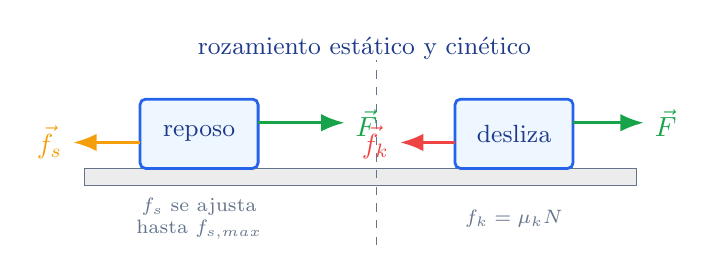
\begin{tikzpicture}[scale=1]
\draw[fill=gray!15, draw=muted] (-.2,0) rectangle (6.8,.22);
\draw[body] (.5,.22) rectangle (2,1.1); \node[text=brand, font=\small] at (1.25,.66) {reposo};
\draw[force,color=accentgreen] (2,.8)--(3.1,.8) node[right] {$\vec F$}; \draw[force,color=accentorange] (.5,.55)--(-.35,.55) node[left] {$\vec f_s$};
\node[sml, align=center] at (1.25,-.42) {$f_s$ se ajusta\\hasta $f_{s,max}$};
\draw[dashed,muted] (3.5,-.75)--(3.5,1.6);
\draw[body] (4.5,.22) rectangle (6,1.1); \node[text=brand, font=\small] at (5.25,.66) {desliza};
\draw[force,color=accentgreen] (6,.8)--(6.9,.8) node[right] {$\vec F$}; \draw[force,color=accentred] (4.5,.55)--(3.8,.55) node[left] {$\vec f_k$};
\node[sml, align=center] at (5.25,-.42) {$f_k=\mu_k N$}; \node[lab] at (3.35,1.75) {rozamiento estático y cinético};
\end{tikzpicture}

\end{document}